\documentclass[11pt]{beamer}
\usetheme{CambridgeUS}
\usepackage[utf8]{inputenc}
\usepackage[english]{babel}
\usepackage{amsmath}
\usepackage{amsfonts}
\usepackage{amssymb}
\usepackage{xcolor}
\usepackage{algpseudocode}
\usepackage{listings}
\usepackage{adjustbox}
\usepackage{subfig}
 
%\definecolor{codegreen}{rgb}{0,0.6,0}
%\definecolor{codegray}{rgb}{0.5,0.5,0.5}
%\definecolor{codepurple}{rgb}{0.58,0,0.82}
%\definecolor{backcolour}{rgb}{1,1,1}
 
%\lstdefinestyle{mystyle}{
%    backgroundcolor=\color{backcolour},   
%    commentstyle=\color{codegreen},
%    keywordstyle=\color{blue},
%    numberstyle=\tiny\color{codegray},
%    stringstyle=\color{codepurple},
%    basicstyle=\ttfamily\footnotesize,
%    breakatwhitespace=false,         
%    breaklines=true,                 
%    captionpos=b,                    
%    keepspaces=true,                 
%    numbers=left,                    
%    numbersep=5pt,                  
%    showspaces=false,                
%    showstringspaces=false,
%    showtabs=false,                  
%    tabsize=2
%}
 
%\lstset{style=mystyle}

\newcommand{\todo}{\textcolor{red}{\textbf{TODO:}}}
\newcommand{\dof}[1]{\begin{itemize}
\item[-]\textcolor{blue}{\textbf{#1 DOFs}}
\end{itemize}}
\newcommand{\norm}[1]{\parallel{#1}\parallel}
\newcommand{\R}{\mathbb{R}}
\newcommand{\diff}[2]{\frac{\partial{#1}}{\partial{#2}}}
\newcommand{\imgG}[3]{\includegraphics[scale={#3}]{../tex/plots/#1/#2}}
\newcommand{\img}[4]{\includegraphics[scale={#4}]{../tex/plots/#1/#2/#3}}

\author[Stefano, Marco]{Stefano De Filippis \& Marco Menchetti}
\title[ROB2 project]{Task priority assignment with collision avoidance}
%\setbeamercovered{transparent} 
%\setbeamertemplate{navigation symbols}{} 
\logo{
\includegraphics[scale=.1]{./images/logo.jpeg}}
\institute[Sapienza]{Sapienza - University of Rome} 
\date{} 
\subject{Robotics II} 
\begin{document}

\begin{frame}
\titlepage
\end{frame}

\begin{frame}{Redundancy resolution problem}
Find Robot command in order to execute a series of tasks. The problem can be formalized as:
\[
Ax = b
\]
with $A = \begin{bmatrix}
A_1^T & A_2^T & \dots & A_l^T 
\end{bmatrix}$ and $
b = \begin{bmatrix}
b_1^T & b_2^T & \dots & b_l^T 
\end{bmatrix}
$.
\[
\sum_{k=1}^{l}m_k \leq n
\]
\end{frame}

\begin{frame}{How to solve redundancy?}
The non prioritized solution is $\overline{x} = A^{\#}b$ if tasks not l.i. we need to accommodate conflicting tasks
\begin{enumerate}
\item Siciliano and Slotine approach: task projection in null space of higher order task
\item Flacco Matrix: separation of redundancy resolution from assignment of correct order
\end{enumerate}
\end{frame}

\begin{frame}{Flacco Matrix}
From base solution we can extrapolate:
\begin{itemize}
\item contribution of each task
\item task null space
\end{itemize}
useful information for reordering.

\textcolor{red}{IDEA:} find a matrix F that allows us to get these information and impose correct priority
\[
x = A^{\#}Fb
\]
\textcolor{red}{RESULTS:} applying F we should get same solution as Siciliano and Slotine.
\end{frame}

\begin{frame}{What is the structure of $F$?}
Generally F has the following structure:
\begin{itemize}
\item It is block lower triangular
\item It has I on diagonal if task l.i. to higher priority task
\item It has 0 blocks on diagonal if task l.d. to higher priority tasks
\item It has coefficient of dependency in the left side of rows
\end{itemize}
\end{frame}

\begin{frame}{How to compute $F$ and final solution?}
We can use Gauss Jordan elimination with pivot square matrices
\begin{columns}
\begin{column}{.5\textwidth}
\begin{block}{Algorithm}
\begin{algorithmic}[1]
\State Use QR decomposition on A $\rightarrow A^{\#} = QR^{-T}$ 
\State Initialize $F$
\ForAll{$row_j$}
\State $row_j \gets P^{\#}*row_j$
\State $row_i \gets row_i - block_{ij}*row_j$ $(i < j)$
\EndFor
\State $F \gets F^T$
\State $x \gets (QR^{-T}*F*b)$
\end{algorithmic}
\end{block}
\end{column}
\begin{column}{.5\textwidth}
\[
\overline{F} = \bordermatrix{
~& m_1 & m_2 & & m_l\cr
m_1 & R_{11} & \star & \dots & \star \cr
m_2 & 0 & R_{22} & \dots & \star \cr
~ & 0 & 0 & \dots & \star \cr
m_l & 0 & 0 & \dots & R_{ll}
}
\]
\end{column}
\end{columns}
\end{frame}

\begin{frame}[fragile]
\frametitle{How to compute $F$: code}
\begin{block}{Code}
\begin{adjustbox}{width=\textwidth , height=.2\textwidth}
\lstinputlisting[language=C++, firstline=98, lastline=113]{../../flaccoController.cpp}
\end{adjustbox}
\end{block}
\end{frame}

\begin{frame}{Why priority?}
\begin{itemize}
\item Decomposition of problems in many tasks.
\item Most problems \textcolor{red}{can't} be solved by just one task.
\item Error is kept on the tasks that \textcolor{red}{can't} be executed	\textbf{EXACTLY} 
\item More natural and smoother behavior.
\end{itemize}
\end{frame}

\begin{frame}{Collision avoidance. How?}
\begin{columns}
\begin{column}{.5\textwidth}
\begin{block}{1. Control points}
Distributing a certain amount of points along the structure of the manipulator we can keep track of its distance from the obstacles and how it changes with respect to the pose.
\end{block}
\begin{block}{2. Collision avoidance}
Whenever a control point is within a certain radius from the surface of the obstacles we start to push it away until we move in a "safe zone".
%\textbf{\textcolor{red}{How do we handle priority?}}
%\begin{itemize}
%\item When the control point is too near the priority lowers (i.e. becomes more important)
%\item As soon as the point exit the \emph{dangerous} region the priority rise again
%\end{itemize}
\end{block}
\end{column}
\begin{column}{.5\textwidth}
\begin{figure}[H]
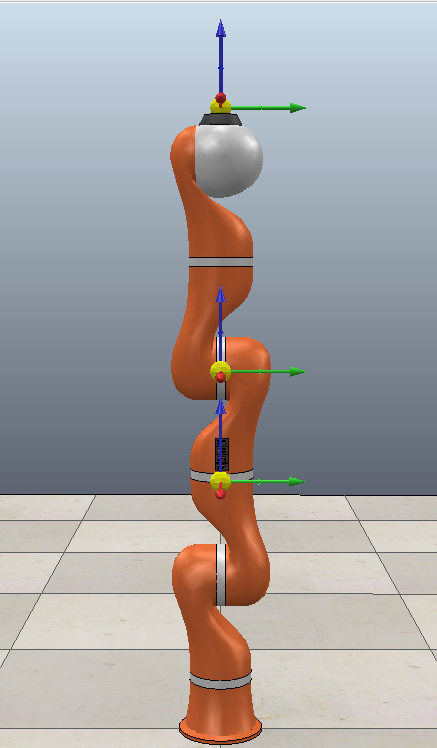
\includegraphics[scale=.25]{./images/KUKA_CPS.png}
\end{figure}
\end{column}
\end{columns}
\end{frame}

\begin{frame}{Collision avoidance. How?}
	\begin{columns}
		\begin{column}{.5\textwidth}
			\begin{block}{2. How do we push?}
			We change approach whether the control point is on the e-e or on the structure:
				\begin{itemize}
				\item For the end-effector we add to the task velocity, a cartesian velocity pointing away from the obstacle.
				\item For the ones on the structure we add the projection of a cartesian velocity, along the distance of the control point from the obstacle (\textcolor{red}{1 DOF}).
				\end{itemize}
			\end{block}
		\end{column}
		\begin{column}{.5\textwidth}
			\begin{figure}[H]
				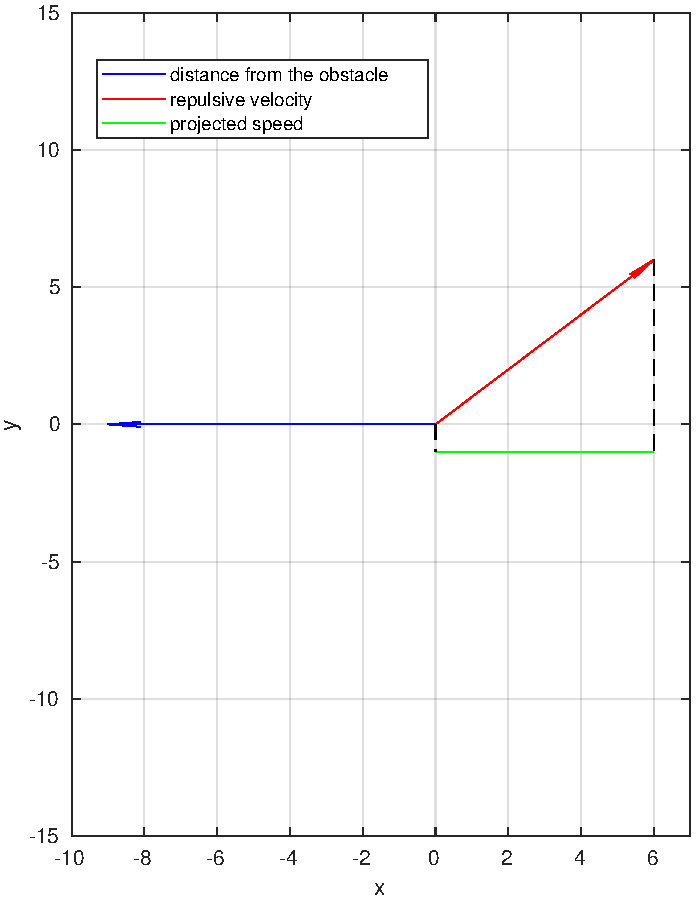
\includegraphics[width = .7\textwidth]{images/repulsive_velocity_vectorial.pdf}
			\end{figure}
		\end{column}
	\end{columns}
\end{frame}

\begin{frame}{Tasks}
We know why to prioritize Tasks, but which are the ones we are going to use?
\begin{itemize}
\item[\textbf{1}] A cartesian positioning task (i.e. we want our e-e to behave in a certain way)
\dof{3}
\item[\textbf{2}] An orientation task used to simulate any kind of auxiliary task
\dof{1}
\item[\textbf{3,4}] Two collision avoidance task, each one on 1 DOF
\dof{2}
\end{itemize}
In the end we saturated 6 out of all the 7 DOFs of the manipulator.
\end{frame}

\begin{frame}{Task 1: Cartesian positioning}
Cartesian positioning means we want the end effector to execute a given trajectory  in $\Bbb R^3$.

\begin{block}{Path used:}
\begin{itemize}
\item A linear path
\item A point-to-point motion path
\end{itemize}
\end{block}

The associated jacobian $J_1$ is the analytical jacobian of the direct kinematics.
\end{frame}

\begin{frame}{Task 1: Collision avoidance}
\begin{itemize}
\item We have \textbf{4} tasks occupying \textbf{6} DOF and we can't another cartesian positioning task. How is it performed?
\end{itemize}
\begin{block}{IDEA:}
Add another repulsive velocity to the desired one, pointing away from the obstacle! 
\end{block}
\begin{itemize}
\item In this way the \emph{Flacco Matrix} will handle the \textcolor{red}{exact} joint velocities so as to execute the \textcolor{red}{sum} of the two.
\item This won't change the jacobian of the task.
\end{itemize}
\end{frame}

\begin{frame}{Repulsive velocity}
\begin{columns}
\begin{column}{.5\textwidth}
\begin{block}{How do we choose?}
We want the repulsive velocity to satisfy a certain amount of properties:
\begin{itemize}
\item Maximum admissible cartesian velocity at distance $d=0$ from the obstacle $\rightarrow V_{max}$.
\item Smooth descending curve $\rightarrow \alpha$.
\item Zero velocity after a given distance from the obstacle $\rightarrow \rho$.
\end{itemize}
\end{block} 
Hence:
\[
v(P,O) = \frac{V_{max}}{1+e^{(\norm{D(P,O)}(2\diagup\rho)-1)\alpha}}
\]
\end{column}
\begin{column}{.5\textwidth}
\begin{figure}[H]
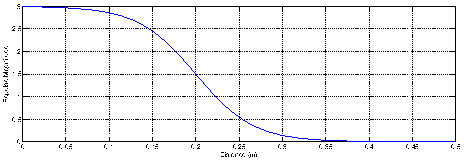
\includegraphics[scale=.45]{./images/repulsive_velocity.pdf}
\end{figure}
\end{column}
\end{columns}
\end{frame}

\begin{frame}{Task 2: Link orientation}
The "orientation task" tries to keep constant the elevation of the third link axis. We need to define it as a vector in $\R^3$:
\[
p_l(q) = p_5(q) - p_4(q)
\]
Applying a coordinate transformation into spherical ones we can easily get the expression of the elevation (dropping the dependencies on $q$):
\[
\phi = \mathrm{arccos}(\frac{p_{l,z}}{\norm{p_l}})
\]
Denoting $p = \frac{p_{l,z}}{\norm{p_l}}$ we can get the expression of the associated jacobian as:
\[
\dot{\phi} = \diff{\phi}{p}\diff{p}{q}\dot{q}
\]
\end{frame}

\begin{frame}{Tasks 3,4: Control points}
\begin{columns}
\begin{column}{.5\textwidth}
We chose the following:
\begin{itemize}
\item The end-effector
\item The origin of the DH reference frame associated with the $4^{th}$ joint
\item The third is on the second link axis at a given distance from the origin of the DH reference frame associated to the 2$^{nd}$ joint (i.e. half link axis' length off the shoulder)
\end{itemize}
\end{column}
\begin{column}{.5\textwidth}
\begin{figure}[H]
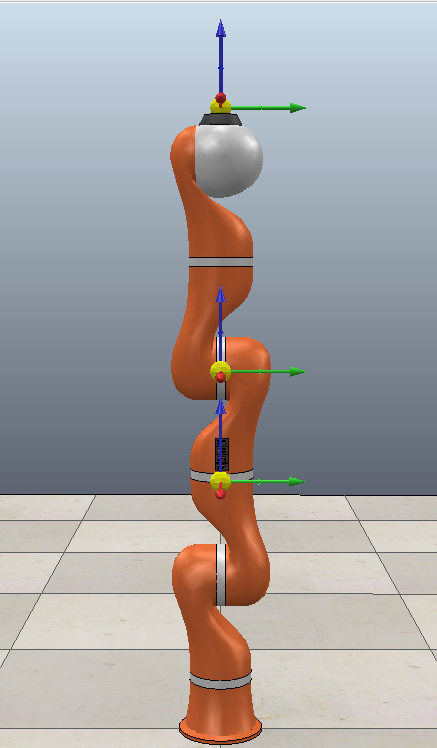
\includegraphics[scale=.25]{./images/KUKA_CPS.png}
\end{figure}
\end{column}
\end{columns}
\end{frame}

\begin{frame}{Tasks 3,4: Collision avoidance}
As already introduced we can't perform collision avoidance for the control points using all the three component of the distance vector. \textcolor{red}{So what?}
\begin{columns}
\begin{column}{.5\textwidth}
\begin{block}{PROJECT!}
We can project the same repulsive velocity we used on task 1, on the distance from the obstacle, obtaining a "repulsive speed" we will call $v$.
\end{block}
\end{column}
\begin{column}{.5\textwidth}
\begin{equation*}
v = \eta^T\dot{r_{o}} = \eta^T J_i\dot{q} = J_{c,i}\dot{q}
\end{equation*}
$J_i$ is the jacobian at the i-th control point.
\end{column}
\end{columns}
\end{frame}

\begin{frame}{Reordering}

\begin{block}{Stack}
We organized the tasks in a vector (here \texttt{stack}) where the first element is the lower priority one and the last is the higher priority one.
\end{block}
This is divided in two parts:
\begin{enumerate}
\item The first part contains the task which are defined \textit{critic}.
\item The second one contains the tasks whose cost is high enough to be in a safe position.
\end{enumerate}

\textcolor{blue}{Criticality}

In order to evaluate which position a task should take within the \texttt{stack}, we need a method to compute a "general cost".
\end{frame}

\begin{frame}{Reordering: cost \& execution}
\begin{columns}

\begin{column}{.4\textwidth}
\begin{itemize}
\item In this application almost each task is associated with a control point so an easy cost function is the minimum distance of the points from the obstacles within the workspace.
\item The second task is not easy to associate a control point with, so we assigned to it a constant cost which is high enough to never make it critical.
\end{itemize}
\end{column}

\begin{column}{.6\textwidth}
The execution of the reordering algorithm is performed as such:
\begin{block}{Algorithm}
\begin{algorithmic}[1]
\ForAll{non critic tasks}
\State reorder by cost
\If{any task cost $\leq$ critic distance}
\State augment number of critic tasks
\EndIf
\EndFor
\ForAll{critic tasks}
\State reorder by cost
\EndFor
\end{algorithmic}
\end{block}
\end{column}

\end{columns}
\end{frame}

\begin{frame}[fragile]
\frametitle{Reordering: code}
\begin{block}{Code}
\begin{adjustbox}{width=.7\textwidth, height=.2\textwidth}
\lstinputlisting[language=C++, firstline=195, lastline=229]{../../flaccoController.cpp}
\end{adjustbox}
\end{block}
\end{frame}

\begin{frame}{Results: angular velocity interesting cases}
\begin{columns}
\begin{column}{.5\textwidth}
\begin{figure}[H]
\img{far}{notAlways}{joint_velocities.eps}{.4}
\caption{obstacle: \textbf{far}, control points not always active}
\end{figure}
\end{column}
\begin{column}{.5\textwidth}
\begin{figure}[H]
\img{far}{always}{joint_velocities.eps}{.4}
\caption{obstacle: \textbf{far}, control points always active}
\end{figure}
\end{column}
\end{columns}
\end{frame}

\begin{frame}{Results: angular velocity interesting cases}
\begin{columns}
\begin{column}{.5\textwidth}
\begin{figure}[H]
\img{on}{notAlways}{joint_velocities.eps}{.4}
\caption{obstacle: \textbf{on}, control points not always active}
\end{figure}
\end{column}
\begin{column}{.5\textwidth}
\begin{figure}[H]
\img{on}{always}{joint_velocities.eps}{.4}
\caption{obstacle: \textbf{on}, control points always active}
\end{figure}
\end{column}
\end{columns}
\end{frame}

\begin{frame}{Results: ee task error in "obstacle on path" case}
\begin{columns}
\begin{column}{.5\textwidth}
\begin{figure}[H]
\img{on}{notAlways}{ee_task_error.eps}{.4}
\caption{obstacle: \textbf{on}, control points not always active}
\end{figure}
\end{column}
\begin{column}{.5\textwidth}
\begin{figure}[H]
\img{on}{always}{ee_task_error.eps}{.4}
\caption{obstacle: \textbf{on}, control points always active}
\end{figure}
\end{column}
\end{columns}
\end{frame}

\begin{frame}{Results: cluttered environment}
\begin{figure}[H]
\label{3obstDist}
\imgG{3obs}{control_points_distances.eps}{.5}
\caption{Control points' distances from $1^{st}$ obstacle}
\end{figure}
\end{frame}
\begin{frame}{Results: cluttered environment}
\begin{figure}[H]
\imgG{3obs}{control_points_distances_2.eps}{.5}
\caption{Control points' distances from $2^{nd}$ obstacle}
\end{figure}
\end{frame}
\begin{frame}{Results: cluttered environment}
\begin{figure}[H]
\imgG{3obs}{control_points_distances_3.eps}{.5}
\caption{Control points' distances from $3^{rd}$ obstacle}
\end{figure}
\end{frame}
\begin{frame}{Results: cluttered environment}
\begin{figure}[H]
\imgG{3obs}{min_3.eps}{.5}
\caption{Minimum distance among all the obstacle}
\end{figure}
\end{frame}

\end{document}